% gscholar.tex
% ─────────────────────────────────────────────────────────────────
% This file defines a single floating figure containing:
%  - (a) a table of Google Scholar metrics
%  - (b) a bar chart of citations per year
%
% It assumes booktabs, pgfplots & subcaption are already loaded.
% ─────────────────────────────────────────────────────────────────

% gscholar.tex
\documentclass[cvauthor={Dr. Sajid Muhaimin Choudhury}]{buetcv}
\begin{document}
\begin{figure}[ht]
    \centering
    % ───── Panel (a): Table ─────
    \begin{subfigure}[t]{0.48\textwidth}
      \centering
      \caption{\aiGoogleScholar Google Scholar Metrics}
      \begin{tabular}{lrr}
        
           &   \\
        \midrule
        Total Citations & 111  \\
        h‑index & 12   \\
        i10‑index & 16   \\
        \bottomrule
      \end{tabular}
    \end{subfigure}\hfill
    % ───── Panel (b): Bar chart ─────
    \begin{subfigure}[t]{0.48\textwidth}
      \small
      \centering
      \caption{\aiGoogleScholar Google Scholar Citations per Year}
      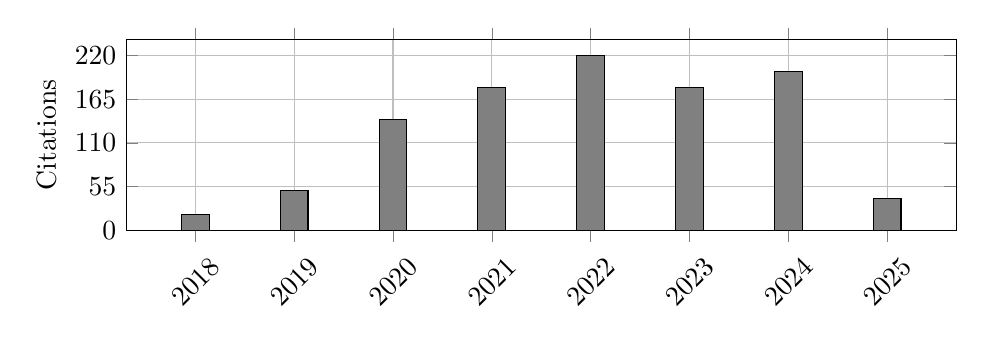
\begin{tikzpicture}
        \begin{axis}[
            width=\linewidth,% make the plot fill the subfigure width...
            height=4cm, % …but only 6 cm tall
            ybar,
            bar width=10pt,
            enlarge x limits=0.1,
            ylabel={\aiGoogleScholar Citations},
            ymin=0, ymax=240,
            ytick={0,55,110,165,220},
            xtick=data,
            xticklabels={2018,2019,2020,2021,2022,2023,2024,2025},
            % rotate the x‐tick labels:
            xticklabel style={rotate=45,anchor=near xticklabel},
            grid=major
          ]
          \addplot[fill=gray] coordinates {
            (2018,20) (2019,50) (2020,140) (2021,180)
            (2022,220) (2023,180) (2024,200) (2025,40)
          };
        \end{axis}
      \end{tikzpicture}
    \end{subfigure}
  \end{figure}
  \end{document}